%\documentclass{acm_proc_article-sp}
\documentclass[a4paper]{article}
\usepackage[a4paper]{geometry}
\usepackage{amsmath}
\usepackage{fontspec}
\usepackage[dvipdfm,colorlinks]{hyperref}
\usepackage{graphicx}
\usepackage{indentfirst}
%\usepackage{multirow}
%\usepackage{bigdelim}


\usepackage{epsfig}
\usepackage{cite}
\usepackage{url}
\usepackage{algorithm}
\usepackage{algorithmic}

\renewcommand{\tablename}{表~}
\renewcommand{\figurename}{图~}
\renewcommand{\refname}{参考文献}
\newtheorem{theorem}{Theorem}

% workaround the old version of alogrithm package
\newcommand{\RETURN}{\STATE {\bf return} }

% chinese settings
\setlength{\parskip}{0.5\baselineskip plus 0.5ex minus 0.2ex}
\XeTeXlinebreaklocale "zh"
\XeTeXlinebreakskip = 0pt plus 1pt minus 0.1pt

% font setting
\setromanfont{SimSun}
% \setsansfont{AR PL New Sung}
% \setromanfont{AR PL ShanHeiSun Uni}

% page settings
\parindent 2em
\topmargin  -1cm
\textheight 23cm
\begin{document}
\title{一种新的动态优先搜索树及其相关算法 \\A Novel Dynamic Priority Search Tree and Its Algorithms}
\date{}
%\author{肖林甫 \quad 陆伟成 \quad 黄惠萍 \quad 赵文庆 \\ 复旦大学专用集成电路与系统国家重点%实验室, 上海, 201203
%\\
%Xiao Linfu \quad Luk Wai-Shing \quad Huang huiping \quad Zhao Wenqing \\ ASIC \& System%State-key Lab, Fudan University, Shanghai, 201203
%\\(0372430@fudan.edu.cn)
%}
\maketitle


\renewcommand{\abstractname}{摘要}
\begin{abstract}
本文提出一种新的、易于实现的动态优先搜索树数据结构及其相关的算法. 它可以应用在交替相移掩模, VLSI版图压缩等VLSI计算机辅助设计领域. 优先搜索树主要是为了进行形如($[x_1:x_2],[-\infty:y]$)的二维查询. 而动态优先搜索树则在维持树的平衡的前提下, 
允许动态的插入和删除节点. 在新的结构下, 所携带的数据只在树的叶结点中. 
它搜索所用的时间是O($\log n+k$), 插入和删除在最坏情况下需要
O($\log n$), 占据的存储空间是O($n$). 其中, $n$是总共节点的个数, $k$是满足搜索条件解的个数.
\end{abstract}

\renewcommand{\abstractname}{Abstract}
\begin{abstract}
A novel dynamic Priority Search Tree (PST) and its algorithms are proposed. It can be applied to the area of computer-aided design such as phase shift masking and VLSI layout compaction.
PST is specialized for 2-D range
query in form of ($[x_1:x_2],[-\infty:y]$). The dynamic PST (DPST) allows dynamic
insertions and deletions while it maintains itself balanced. A
DPST takes O($\log n+k$) time for quary. Insertion and
deletion have worst case requirements of O($\log n$), occupied
O($n$) storage space, respectively, where $n$ is the total number of
nodes in the tree, and $k$ the number of solutions in query.
\end{abstract}


\section{导言}

优先搜索树(Priority Search Tree)提出于80年代~\cite{CG_01},然而, 跟kd-tree, quad-tree相比~\cite{CG_03}, 它并没有在电子设计自动化(EDA)领域受到广泛的注意.  
原因之一是优先搜索树的实现比较复杂, 尤其是还需要动态平衡的时候. 
另一个的原因则可能是其特殊的区域查找, 使得它不能用于一般的应用. 但是, 动态优先搜索树(Dynamic PST)可以应用在寻找相交的矩形, 构造冲突图当中, 下面我们先来介绍一下它的应用.

\subsection{应用}
动态优先搜索树(DPST)主要的应用是为了存储线段集合, 因为数轴上的线段可以与平面上的点一一对应起来, 搜索相交的线段就相当于做一次类似($[x_1:\infty],[-\infty:y]$)的二维搜索~\cite{GG}. 
\subsubsection{矩形相交}
为了探测出平面上所有与xy轴平行的矩形之间的相交关系, 我们可以采用平面扫描算法~\cite{CG_02}, DPST用作中间数据结构来存放线段集合. 

    平面扫描算法是假想有一条直线, 垂直于x轴从左至右将平面上的图形扫一遍. 与扫描线相交的所有矩形构成的集合, 称为扫描线的状态, 随着扫描线的向右推进, 其状态不断变化, 但其变化不是连续的, 只有在某些特定的位置, 才需要对扫描线的状态进行更新. 我们称这些位置为平面扫描算法的事件点. 就本算法而言, 事件点是各矩形在x轴上投影的端点. 

    只有扫描线触及某个事件点时, 算法才会进行实质的处理. 更新扫描线的状态, 并进行一些相交测试. 具体的, 若事件点为矩形的左端点, 则意味着这个矩形开始与扫描线相交, 因此需要将该矩形插入到某状态结构中. 然后需要将这个矩形和那些与当前扫描线相交的其他矩形测试, 确定是否相交. 若事件点为矩形的右端点, 则将矩形从状态结构中删去. 这样扫描一遍, 即可找出所有相交的矩形. 

    上述的状态结构, 我们可以用DPST来实现. 矩形在y轴上投影的线段$[y_1, y_2]$, 都可以对应成平面上的点$(y_2, y_1)$. 设与当前扫描线相交的所有矩形在y轴上的投影的线段集合为$I:=\{[x_1,y_1],[x_2,y_2],\ldots,[x_n,y_n]\}$, 对应为DPST里的点集
$K:=\{(y_1, x_1),(y_2, x_2),\ldots,(y_n, x_n)\}$.
当我们测试当前矩形和那些在状态结构中的矩形是否相交的时候, 实际上, 就是测试当前矩形的y线段$[y_{m1}, y_{m2}]$, 与线段集合$I$中的线段是否相交, 也就是相当于在DPST中找出所有在$([y_{m1}:\infty],[-\infty:y_{m2}])$区域内的点. 这正是动态优先搜索树所能做的. 如图1所示, 它是把所有矩形扩大某个长度$d$后, 再进行矩形相交检测, 所得到的结果. 两个矩形之间有线段连接表示它们扩大长度$d$后会相交.
\begin{figure}[!h]
  \centering
  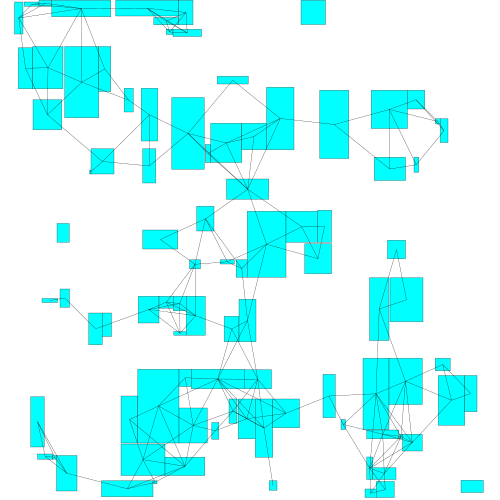
\includegraphics[scale=0.5]{conflict.pdf}\\
  \caption{冲突图}\label{fig:conflict}
\end{figure}

\subsubsection{具体应用}
    在全局布线, VLSI版图压缩~\cite{DAC_05}以及动态路由表~\cite{xx_05}~\cite{ISCC_05}, 都用到了PST. 在交替相移掩模(Phase Shift Masking~\cite{PSM_05})中, 我们构造冲突图, 也是要读入一个版图文件, 探测各个结构之间的相交关系, 这时也可以用到DPST. 在纳米技术工艺下, 由于光的衍射导致光刻掩模版上本来应该是没有光照的地方, 却有了光强. 导致照出来的图形, 与光刻掩模版上的图形有出入. 于是出现了像光学近似校正(Optical Proximity Correction), 交替相移掩模(PSM)技术. 交替相移掩模是让那些靠的很近足以产生强衍射的光束能够分配到不同的相位, 这样原来的干涉相长, 就变成了干涉相消. 于是上述问题就解决了. 我们把所有需要分配不同相位的图形找出来, 就形成了冲突图. 然后我们根据权重, 分配相位. 图2是某个版图已经分配好相位的例子. 红色绿色代表不同的相位, 灰色代表随意分配相位.

    PSM中, 构造冲突图是关键的一步. 我们读入一个大的GDSII版图文件, 先将版图中所有的多边形全部切割成矩形, 然后将其扩大, 扩大的长度就是光能衍射出来的宽度. 扩大后如果矩形相交了, 说明他们需要分配不同的相位. 我们把所有需要分配不同相位的图形用边联系起来, 这样就构成了冲突图. 构造冲突图的问题, 转化为寻找所有相交的矩形的问题. 而这个问题可以选择用1.1.1所述的平面扫描算法+动态优先搜索树解决. 

\begin{figure}[!h]
  \centering
  \includegraphics[scale=4]{assignment.pdf}\\
  \caption{相位分配}\label{fig:assignment}
\end{figure}


\subsection{优先搜索树简介}
给定一个二维的点(x,y)的集合, 优先搜索树将这些数据按一定规则组织到一个二叉搜索树之中. 
优先搜索树整合了两种数据结构于一体: 一维区域树和堆. 
它主要是为了形如($[x_1:x_2],[-\infty:y]$)的二维查询. 而平衡的动态优先搜索树则是在RB-tree或者是AVL-tree基础上的一个扩展. 在我们的版本中, 数据只存放在叶节点中, 
这也是我们与前人版本的不同关键之处. 请看图3. 
我们用叶结点存储数据, 用内节点存储
搜索用的信息. 
每一个内部节点包含了其所有子树所有节点的x坐标的中间值--这看起来像一个一维区域树; 
同时, 每一个内部节点还包含了其所有子树所有节点的y坐标的最小值
--这看起来又是一个堆. 

优先搜索树 = 一维区域树 + 堆



\subsection{新版本的优点}
80年代McCreight提出关于优先搜索树和动态优先搜索树的概念和实现~\cite{Edward_04}, 至今人们的实现都是基于他的思想. 但是, 动态优先搜索树复杂的设计, 
以致于实现起来比较困难. 一位Linux内核的开发人员曾经在写道~\cite{LNX_03},
"我们本来可以使用一个平衡的动态优先搜索树来优化树的高度, 
但是~\cite{Edward_04}提出的版本对于我们的用途来说实现起来太复杂太耗内存了."
本文提出一个实现起来比较容易的方法. 
而且我们把旋转的时间复杂度从O($\log(n)$)降到了常数. 这样一来, 
插入和删除节点的时间上也会有所改进. 

另外, 以前的版本在查询的时候, 用了递归的方法, 并且返回的是一个所有解的数组. 
我们在此作了改进, 我们返回的是一个迭代器(iterator), 每次调用iterator++返回下一个解. 就像C++里STL(Standard Template
 Library)里面的风格一样, 
这样使用起来更加的方便. 相比较而言, 这样遍历解需要消耗时间会多一些. 
这是因为我们把数据总存储在叶节点中, 这当然就要比存储在内部节点的数据更晚一些被探测到. 

虽然如此, 这样的利弊得失在EDA的物理设计领域还是很有意义的. 在VLSI物理设计中, 
我们常常要读入版图文件, 然后计算出里面图形之间的位置关系, 比如是否相交等等. 
普遍的方法是采用平面扫描算法, 由于版图文件的巨大, 通常都有几百兆. 
如果用动态优先搜索树来做中间数据结构的话, 处理的速度会有很大提高. 
在实际应用中, 我们会频繁的向中间数据结构来作插入和删除, 而每次查询搜索
得到的解都是比较少的. 这样, 跟以前的版本相比, 总体来说我们版本的动态优先搜索树
较之前版本要快. 

\section{预备知识}
%\subsection{一维区域树~\cite{CG_03}和堆}
图3是我们的PST:
\begin{figure*}[!h]
  \centering
  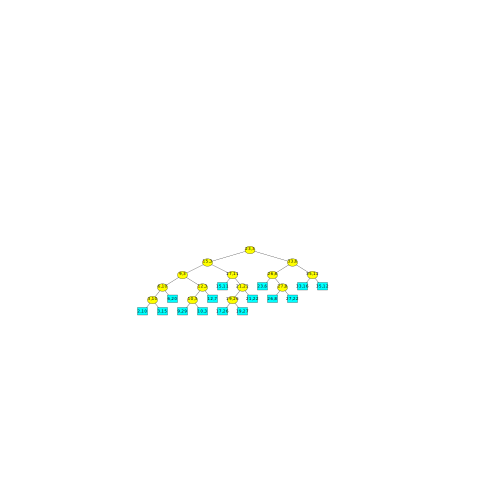
\includegraphics[scale=0.5]{pst.pdf}\\
  \caption{优先搜索树.}\label{fig:pst}
\end{figure*}

只看节点的第一个坐标, 这是一个一维区域树. 
给定一个实数的集合$P:=\{x_1,x_2,\ldots,x_n\}$, 我们可以用平衡二叉搜索树$T$来建立
一个一维区域树. 用叶节点存储整个集合$P$, 用内节存储用来引导搜索的中间键值. 我们
假设内节点$v$存储中间键值为$x_v$, 那么存储在其左子树节点上的值都严格比$x_v$小,
而存储在其右子树节点上的值都大于或等于$x_v$.

像STL's set$<>$, multi-set$<>$, map$<>$. 都是基于一维区域树来实现的. 


见图3, 只看节点的第二个坐标, 我们发现这就是一个堆. 堆是一种
常见的数据结构, 此不赘述. 


%\section{问题定义}
PST可以用来解决以下的问题:\\
给定平面上的点的集合$K:=\{(x_1,y_1),(x_2,y_2),\ldots,(x_n,y_n)\}$, 
我们要找出所有满足区域搜索条件($[x_a:x_b],[-\infty:y]$)的所有点的集合, 
并且可以动态向$K$中插入或是删除一个点$(x_m,y_m)$. 


\section{节点数据结构}

节点定义如下: 
\begin{verbatim}
Node v 	{
    Point p;
    Node *left, *right, *parent;
    Bool winner;
    Nodecolor color;
}
\end{verbatim}

我们把数据(点)集合$K$中的所有数据都存储在叶节点的成员$p$中, 
而内节点只存放搜索用的信息. 动态优先搜索树中所有内节点的左,右子节点都非空, 集合中有$n$个点, 
则DPST则含有$2n+1$个节点, 而一棵Radix-PST~\cite{Edward_04}(一种不平衡的动态优先搜索树)只含有$n$个节点. 
叶节点中的成员$p$按照$p.x$的顺序从左到右,从小到大排列. 
内节点中, $p.x$用来存储其子树中关于$x$坐标的中间键值, 也就是其前序遍历后节点的$p.x$值. 
$p.y$用来存储其子树中$y$坐标的最小的节点的$p.y$值. 

请看图3, 每一个节点$v$中, 我们画出了$p.x \& p.y$, 对于$v.p.x$来说, 这个
数据结构是一个一维区域树; 对于$v.p.y$来说, 这个数据结构是一个堆. 

我们可以用类似锦标赛的方法来构造这个堆. 自底而上, 每个节点的左,右子节点进行比赛.
谁的$p.y$小谁就获胜, 晋级到下一轮. 并且让其成员$winner$为真, 反之, 则为假. 见算法1.

我们之所以在结点中保留$winner$这样的布尔值, 是为了在插入和删除节点进行锦标赛时,
可以利用到原来的结点间的胜负关系, 使比较次数尽可能少. 简而言之, 就是如果你赢了
A, 那么你一定可以赢那些输给A的人, 如果你输给了A, 那么你一定会输给那些赢A的人. 

成员$left, right, parent$的意义不言而喻, 分别是指向其左,右,父节点的指针. $color$则是
红黑树当中的平衡因子. 

\begin{algorithm}[!h]
\caption{锦标赛} \label{alg:tournament}
	\begin{algorithmic}[1]
	\REQUIRE PST节点$v$
	\STATE $v.p.y$ $\leftarrow$ 最小值($v.left.p.y$, $v.right.p.y$)	
	\IF{$v.left.p.y$ $<$ $v.right.p.y$}
	\STATE $v.left.win$ $\leftarrow$ True
	\ELSE
	\STATE $v.left.win$ $\leftarrow$ False
	\ENDIF
	\STATE $v.right.win$ $\leftarrow$ ! $v.left.win$
	\end{algorithmic}
\end{algorithm}




\section{插入节点}

插入算法分为两大步, 见算法2. 设新的点为$(x_1,y_1)$. 首先, 找到新点待插入的位置.
我们知道, 一个优先搜索树只看成员$p.x$的话是一个二叉树. 所以我们从根节点开始,
自顶而下, 如果$x_1$比内节点的$p.x$小的话, 则走向往该内节点的左节点. 反之, 走向
右节点. 直到碰到叶节点为止. 设那个叶节点为$v$. 然后创建一个新节点$z$, 并用其代替$v$.
再创建一个新节点$w$, 让其$p$的值为$(x_1,y_1)$. 让$v$和$w$成为$z$的子节点. 
见图4, 是将点$(18,5)$插入到图3所示PST的情景. 此时, $v$是$(17, 26)$, $w$是$(18,5)$

\begin{algorithm}[!h]
\caption{插入算法} \label{alg:pst_insert}
    \begin{algorithmic}[1]
     \REQUIRE DPST $T$ 和点 $(x_1,y_1)$. 
     \STATE 根据$x_1$的值找到待插入的节点. 设为$v$.
     \STATE 创建一个新节点$z$, 并用其代替$v$.
     \STATE 创建一个新节点$w$, 让其$p$的值为$(x_1,y_1)$.
     \STATE 让$v$和$w$成为$z$的子节点.
     \STATE 维持区域树的特性.
     \STATE 维持堆的特性. 
     \COMMENT {以上步骤的时间复杂度O($\log n$).}
     \STATE 平衡这棵树$T$.
     \COMMENT {这步时间复杂度O($\log n$). 详细的讨论在重新平衡章节.}
    \end{algorithmic}
\end{algorithm}

\begin{figure*}[!h]
  \centering
  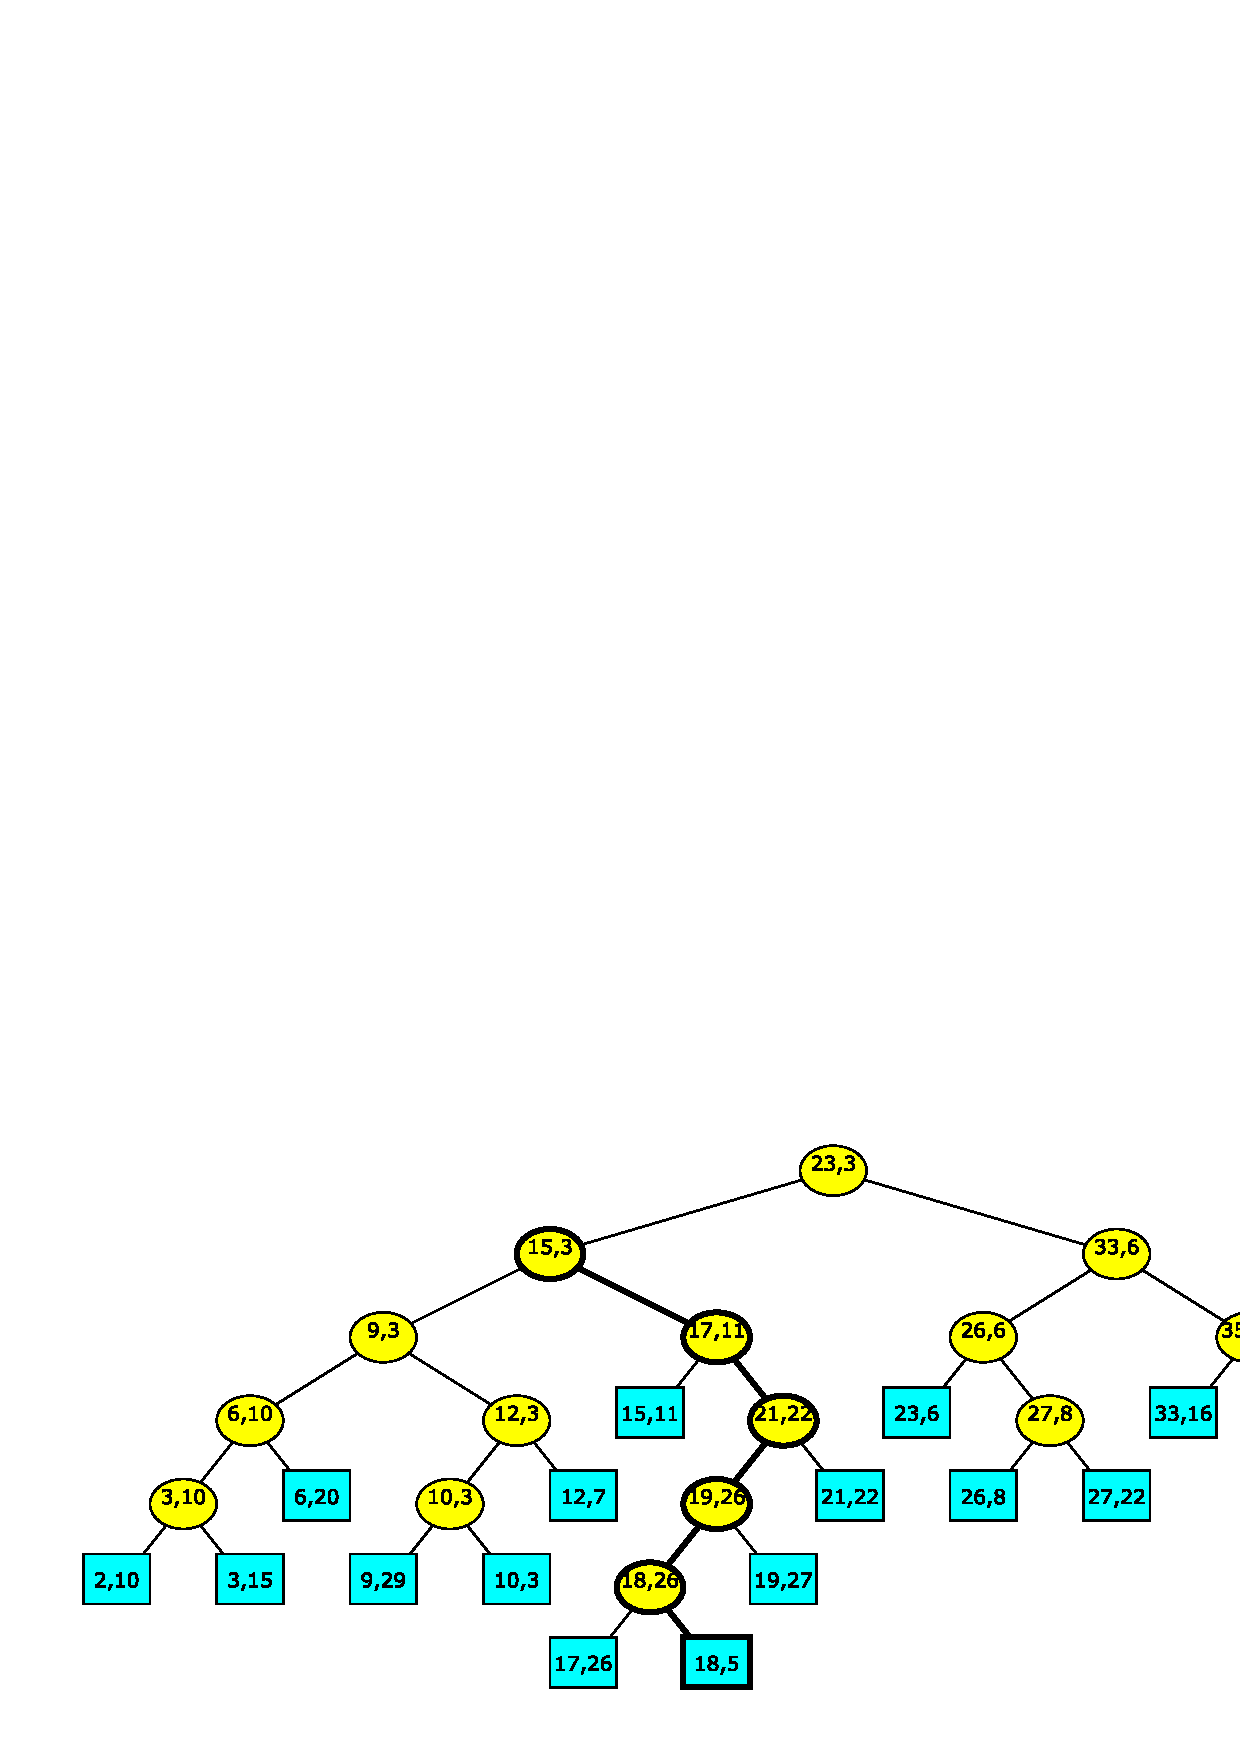
\includegraphics[scale=0.5]{pst_just_insert.pdf}\\
  \caption{插入节点: 锦标赛之前.}\label{fig:pst_just_insert}
\end{figure*}

第二步, 我们要更新内节点的$p$值来维持住DPST的一维区域树和堆的特性. 
对于$p.x$值, 总共只有两个节点需要更新. 一个是$z$, 另一个是$z$的右节点的前序遍历后节点.
算法如下:


\begin{algorithm}[!h]
\caption{维持区域树的特性} \label{alg:rangetreefeature}
	\begin{algorithmic}[1]
	\STATE $z.p.x$ $\leftarrow$ $z.right.p.x$
	\STATE $tmp$ $\leftarrow$ $z.left$
	\WHILE{$tmp$ 不是根节点 并且 $tmp$ 是其父节点的左节点}
	\STATE $tmp$ $\leftarrow$ $tmp.parent$
	\COMMENT {寻找$z$的右节点的前序遍历后节点}
	\IF{$tmp$ 不是根节点}
	\STATE $tmp.parent.p.x$ $\leftarrow$ $z.left.p.x$
	\ENDIF
	\ENDWHILE
	\end{algorithmic}
\end{algorithm}

对于$p.y$值, 从$z$节点开始进行锦标赛, 尽量利用winner来减少比赛次数.
当其输给其兄弟节点时锦标赛结束. 见图5. 

\begin{figure*}[!h]
  \centering
  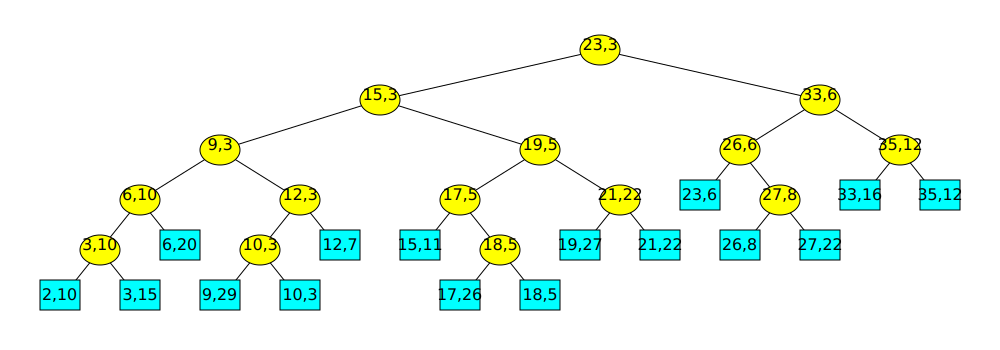
\includegraphics[scale=0.5]{pst_insert.pdf}\\
  \caption{插入: 锦标赛和平衡之后}\label{fig:pst_insert}
\end{figure*}

插入节点的时间复杂度为O($\log n$). 


\section{删除节点}

删除的算法与插入的算法类似, 做一些反方向的工作. 见算法4. 

\begin{algorithm}[!h]
\caption{删除节点} \label{alg:pst_delete}
    \begin{algorithmic}[1]
    \REQUIRE DPST $T$ 和点 $(x_1,y_1)$. 
    \STATE 用二叉查找找到待删除的节点$v$. 设$z$是$v$的父节点, $w$是$v$的兄弟节点.
    \STATE 用$w$替换$z$.删除$v$, $z$.
    \STATE 维持区域树的特性.
    \STATE 维持堆的特性. 
    \COMMENT {以上步骤的时间复杂度O($\log n$).}
    \STATE 平衡这棵树$T$.
    \COMMENT {这步时间复杂度O($\log n$). 详细的讨论在重新平衡章节.} 
    \end{algorithmic}
\end{algorithm}
删除节点的时间复杂度为O($\log n$).

\section{查询}
在解决($[x_1:x_2],[-\infty:y]$)的区域查询的问题上我们可以有两种
不同的思路: 一种是用递归的算法\cite{CG_03}, 最后返回一个点的数组, 另一种采用类似STL中迭代器的方法, 每次先返回一个解的指针(iterator), 然后用iterator++的方法遍历整个数组. 我们采用的是后一种, 这也是我们
跟先前版本的不同之处.

\subsection{迭代器方法}
DPST的迭代器数据结构如下, 这个迭代器与其他普通的迭代器的不同之处是, 它不仅存储了节点的指针, 还有一个y坐标值.
\begin{verbatim}
iterator{
    Node * node;
    int y;
}
\end{verbatim}

LowerBound()函数返回了一个迭代器$iterator$, 这个迭代器指向在树中最左边的一个满足条件的节点. 
并且执行$iterator$++的时候, 返回右边的下一个. UpperBound()函数也返回一个迭代器$iterator$, 这个迭代器指向在树中最右边的一个满足条件的节点. 并且执行$iterator$--的时候, 返回左边的前一个. 
于是, 我们从一边出发, 用类似算法5的方法就可以遍历整个解. 

\begin{algorithm}[!h]
\caption{遍历整个解} \label{alg:traversing}
	\begin{algorithmic}[1]
	\STATE $it1$ $\leftarrow$ LowerBound($v$,$x_1$,$x_2$,$y$)
	\STATE $it2$ $\leftarrow$ UpperBound($v$,$x_1$,$x_2$,$y$)
	\REPEAT
	\STATE 做一些我们需要的处理
	\STATE $it1$++
	\UNTIL{$it1==it2$} 
	\end{algorithmic}
\end{algorithm}

LowerBound()设计, 见算法5, 6. UpperBound()的代码与此类此.

\begin{algorithm}[!h]
\caption{LowerBound} \label{alg:find lowerbound}
    \begin{algorithmic}[1]
    \REQUIRE 一个PST $T$ 和 三个值$x_1,x_2$ 且
$x_1<x_2$, $y$
    \STATE 从根节点开始, 用二分法找到第一满足$p.x$坐标在$x_1,x_2$之间的节点$v$
    \RETURN iterator(LowerBoundRecur($v$,$x_1$,$x_2$,$y$), $y$)
    \end{algorithmic}
\end{algorithm}

\begin{algorithm}[!h]
\caption{LowerBoundRecur} \label{alg:find lowerboundrecur}
    \begin{algorithmic}[1]
    \REQUIRE 一个PST $T$ 和 三个值$x_1,x_2$ 且
$x_1<x_2$, $y$
    \STATE $tmp$ $\leftarrow$ NULL
    \WHILE {$v$ 不是 null}
	\IF{$y<v.p.y$}
        \RETURN $tmp$ //没找到
        \ENDIF
        \IF{v 是叶节点}
            \IF{!$(v.p.x<x_1)$ 并且 !$(v.p.x>x_2)$}
                \RETURN $x$ //找到了
	    \ELSE
                \RETURN $tmp$ //没找到
            \ENDIF
	\ENDIF
	\IF{!$(v.p.x < x_1$)}
	\STATE $tmp$ $\leftarrow$ LowerBoundRecur($v$,$x_1$,$x_2$,$y$);
	\ENDIF
	\IF{$tmp$ 不是 null}
            \RETURN $tmp$ //找到了
        \ENDIF
	\STATE $v$ $\leftarrow$ $v$的右子节点
	\ENDWHILE
     \RETURN $tmp$
\end{algorithmic}
\end{algorithm}

接着, 我们再看看关于迭代器自增的算法, 见算法8, 算法9. 

\begin{algorithm}[!h]
\caption{operator$++$} \label{alg:operator++}
	\begin{algorithmic}[1]
	\REQUIRE 一个PST的迭代器$it$
	\REPEAT
	\STATE increment($it$)
	\IF{$it.node$ 是 null}
	\STATE Break
	\ENDIF
	\UNTIL($it.node$ 是叶节点 并且 $it.node.y <= y$)
	\end{algorithmic}
\end{algorithm}

\begin{algorithm}[!h]
\caption{increment($iterator$)} \label{alg:increment}
	\begin{algorithmic}[1]
	\REQUIRE 一个PST的迭代器$it$
	\IF{$it.node$ 是叶节点}
		\WHILE{$it.node$ 是其父节点的右子节点 并且 $it.node$ 不是根节点}
		\STATE	$it.node$ $\leftarrow$ (it.node 的父节点)
		\ENDWHILE
		\STATE	$it.node$ $\leftarrow$ (it.node 的父节点)
	\ELSE
		\STATE	$it.node$ $\leftarrow$ (it.node 的右子节点)
		\WHILE{$it.node.y >= it.y$ 并且 $it.node$ 不是叶节点}
		\STATE	$it.node$ $\leftarrow$ (it.node 的左子节点)
		\ENDWHILE
	\ENDIF
	\end{algorithmic}
\end{algorithm}

\section{重新平衡树}
请注意, 由于我们的DPST只是平衡二叉树的的推广, 所以我们只要修改原来红黑树旋转部分的代码就可以了. 
\subsection{旋转}
对红黑树而言, 插入和删除操作中, 结点可能被旋转以保持树的平衡. 此外, 由于它的设计, 任何不平衡都会在三次旋转之内解决.
在旋转前后, 一维区域树的特性并没有改变, 对内节点中的$p.x$值不需要调整. 但是堆的特性却被破坏了, 因此我们要在
旋转的同时调整一下内节点中的$p.y$的值, 来维持堆的特性. 以下各图中,节点内只画出了$p.y$的值. 

不失一般性, 我们只列出顺时针旋转的情况. 用$x, y$来表示待旋转的节点, 其中$y$是$x$的右节点.
用$ly, ry$表示$y$的左右节点, 用$lx, rx$表示$x$的左右节点, 一共可以分为下列二大类情况. 

情况1: 在锦标赛中$y$是输家. 

可以推出$lx$必然赢家, 而且旋转之后, 各节点的胜负关系不会变, 见图6情况1, 
旋转结束, 该情况只消耗常数时间.
\begin{figure}[!h]
  \centering
  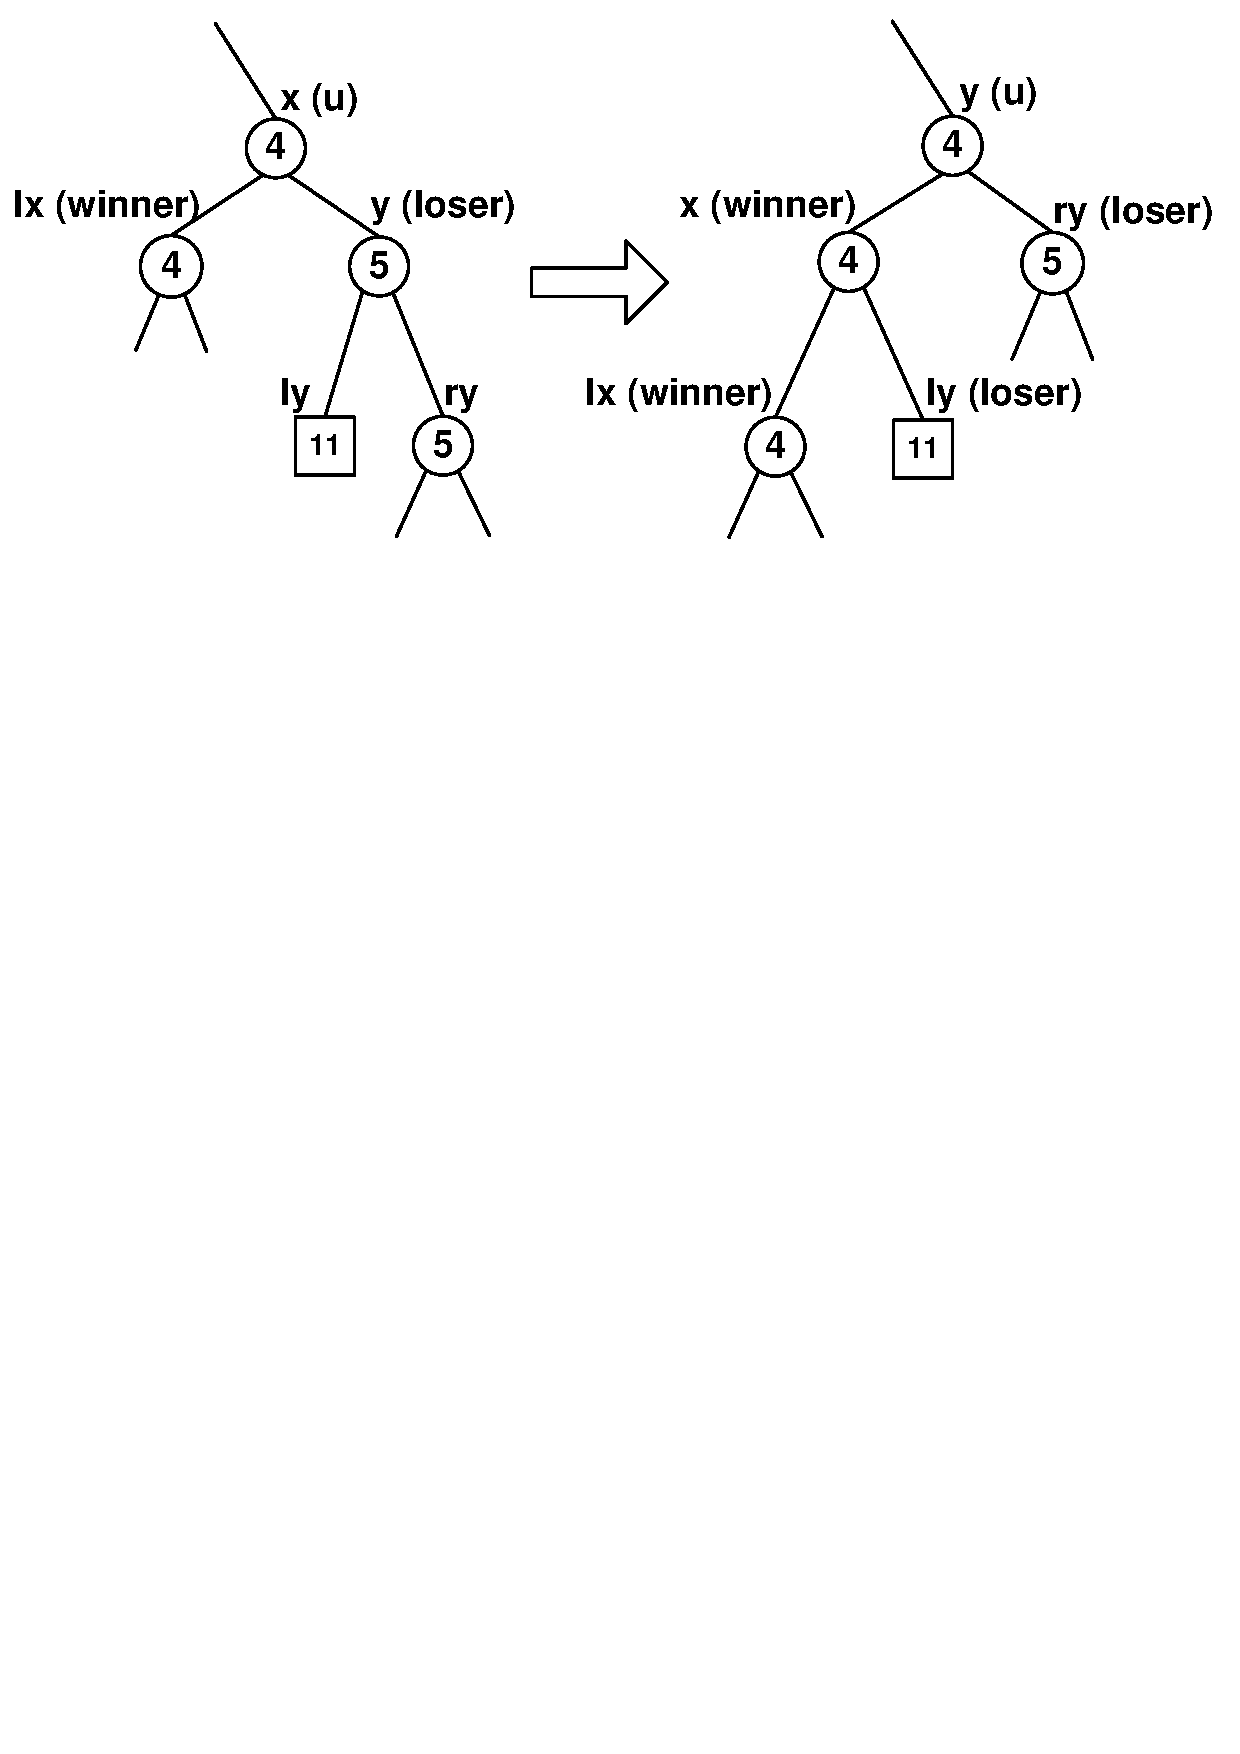
\includegraphics[scale=0.4]{case_1.pdf}\\
  \caption{情况1.}\label{fig:case_1}
\end{figure}

情况2: 在锦标赛中$y$是赢家. 

情况2.1: $ly$是赢家. 图7情况2.1. 可推出$x$也是赢家.
旋转后各个节点的状态没有发生改变, 旋转结束, 消耗常数时间.
\begin{figure}[!h]
  \centering
  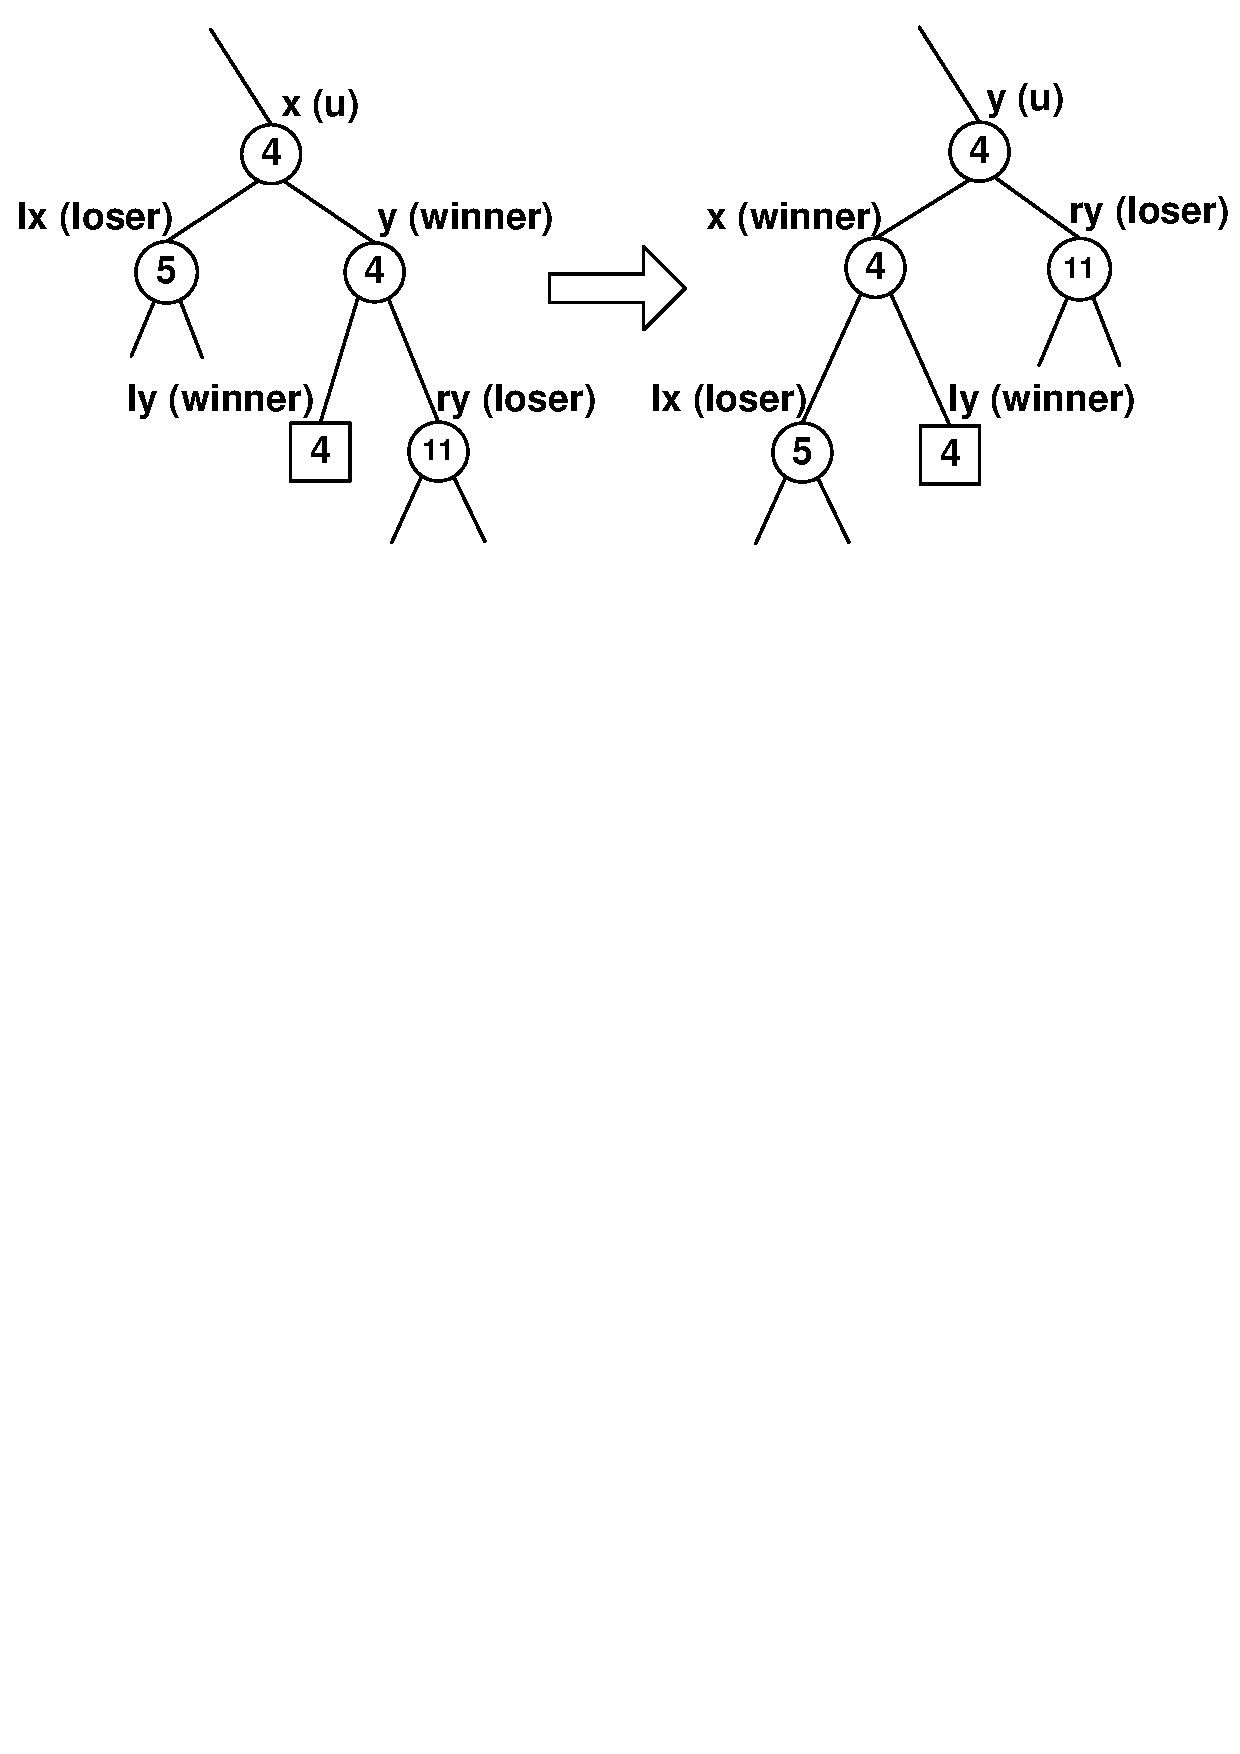
\includegraphics[scale=0.4]{case_2_1.pdf}\\
  \caption{情况2.1.}\label{fig:case_2_1}
\end{figure}

情况2.2: $ly$是输家. 图8情况2.2. 可推出$lx$和$ly$都$>=4$,
$ry$也将是赢家. 旋转后还需进行一次$lx$与$ly$的重赛. 但即使是这样, 消耗时间也是常数.

\begin{figure}[!h]
  \centering
  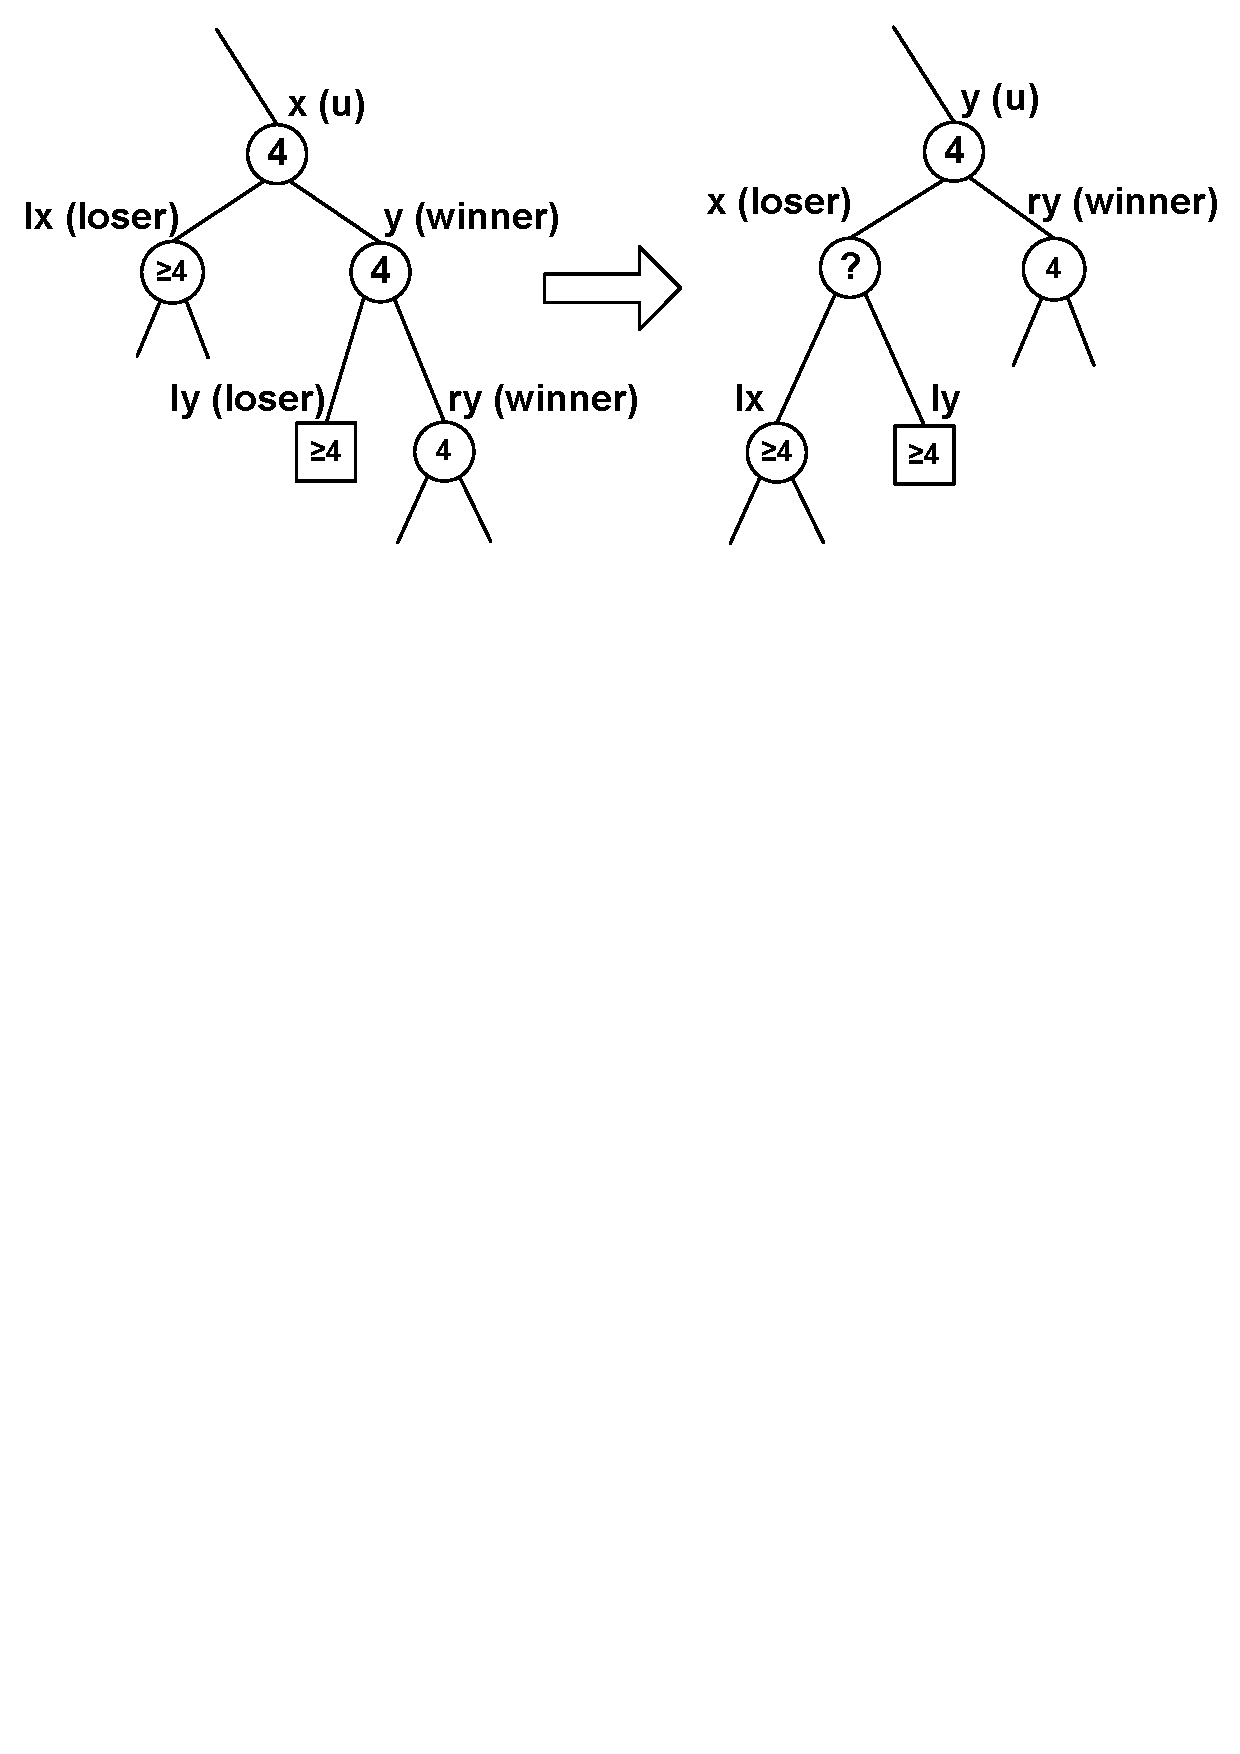
\includegraphics[scale=0.4]{case_2_2.pdf}\\
  \caption{情况2.2.}\label{fig:case_2_2}
\end{figure}
\end{proof}

综上所述, 我们的结论是, DPST一次旋转的时间复杂度的常数.

\subsection{插入和删除的时间复杂度}
总而言之, 一次旋转的时间是O(1), 而以前的版本~\cite{Edward_04}在最坏情况下要O($\log n$),
原因是它要从当前节点向叶节点方向更新内节点的值. 在一次插入或删除的过程中, 
如果我们用红黑树来作为平衡因子, 最多需要旋转3次, 原版本和新版本的时间复杂度都是O($\log n$). 
但是我们新版本的时间开销要小. 

\section{实验结果}

这一节中, 我们将做一些实验, 来验证我们的理论. 实验环境是一台linux服务器, 硬件条件
是2.80GHz Intel(R) Xeon(TM) CPU, 8GB内存. 
我们实现了两种平衡的动态优先搜索树, 新版本和以前的版本~\cite{Edward_04}. 并且还实现了
一个非平衡的动态优先搜索树Radix PST (RPST)~\cite{Edward_04}. 我们将同时比较这三种数据结构在插入, 删除和查询时的运行时间. 

\subsection{插入}
我们比较两个时间, 一个是创建整棵树所用的时间, 还有一个是创建整棵树后, 再向其插入10个节点所用的时间. 我们先选一些在平面上分布均匀的点来做实验. 
\begin{table}[ht]
\centering
\begin{tabular}{|p{1.1cm}|p{0.8cm}|p{0.8cm}|p{0.8cm}|p{0.8cm}|p{0.8cm}|p{0.8cm}|}
\hline 节点 & \multicolumn{3}{|c|}{插入10个点($\mu$s)} & \multicolumn{3}{|c|}{总共运行时间(ms)}\\
\cline{2-7}
个数 & 新 DPST & 原 DPST  & RPST & 新 DPST & 原 DPST & RPST\\
\hline 1000 & 5 & 6 & 9 & 0.5 & 0.66 & 0.3\\
\hline 5000 & 14 & 16 & 5 & 3.0 & 4.1 & 1.7\\
\hline 10000 & 8 & 9 & 5 & 6.6 & 8.8 & 3.7\\
\hline 50000 & 14 & 28 & 7 & 62 & 116 & 25\\
\hline 100000 & 17 & 22 & 10 & 143 & 183 & 66\\
\hline 500000 & 26 & 60 & 17 & 1186 & 1342 & 572\\
\hline
\end{tabular}
\caption{插入(均匀取点)}
\end{table}

我们再选一些在平面上分布不均匀的点来做实验, 让大部分点都来自一个很窄的区间.

\begin{table}[ht]
\centering
\begin{tabular}{|p{1.1cm}|p{0.8cm}|p{0.8cm}|p{0.8cm}|p{0.8cm}|p{0.8cm}|p{0.8cm}|}
\hline 节点 & \multicolumn{3}{|c|}{插入10个点(us)} & \multicolumn{3}{|c|}{总共运行时间(ms)}\\
\cline{2-7}
个数
& 新DPST & 原DPST  & RPST & 新DPST & 原DPST & RPST\\
\hline 1000 & 5 & 6 & 11 & 0.49 & 0.67 & 0.56\\
\hline 5000 & 11 & 8 & 5 & 2.9 & 4.0 & 2.2\\
\hline 10000 & 7 & 11 & 5 & 6.6 & 8.8 & 5.2\\
\hline 50000 & 13 & 23 & 28 & 57 & 75 & 60.8\\
\hline 100000 & 16 & 19 & 61 & 137 & 180 & 294\\
\hline 500000 & 28 & 29 & 369 & 1082 & 1377 & 9146\\
\hline
\end{tabular}
\caption{插入(非均匀取点)}
\end{table}

从这里我们可以看出, 不管怎样取点, 我们的新版本DPST的速度都比原版本DPST的快. 但是对于RPST, 由于它不是一颗平衡的树, 所以在不同的情况下表现很不一样, 分布均匀的时候很快, 但是不均匀时导致树严重不平衡, 故速度很慢. 

\subsection{删除}
我们比较两个时间, 一个是删除整棵树所用的时间, 还有一个是建立整棵树后, 再向其删除10个节点所用的时间. 我们先选一些在平面上分布均匀的点来做实验. 

\begin{table}[ht]
\centering
\begin{tabular}{|p{1.1cm}|p{0.8cm}|p{0.8cm}|p{0.8cm}|p{0.8cm}|p{0.8cm}|p{0.8cm}|}
\hline 节点 & \multicolumn{3}{|c|}{删除10个点(us)} & \multicolumn{3}{|c|}{总共运行时间(ms)}\\
\cline{2-7}
个数 & 新DPST & 原DPST  & RPST & 新 DPST & 原DPST & RPST\\
\hline 1000 & 7 & 9 & 5 & 0.29 & 0.4 & 0.2\\
\hline 5000 & 9 & 11 & 8 & 1.90 & 2.5 & 1.3\\
\hline 10000 & 13 & 18 & 6 & 6.56 & 6.7 & 2.9\\
\hline 50000 & 21 & 40 & 13 & 56.2 & 87.0 & 24.1\\
\hline 100000 & 26 & 28 & 18 & 143 & 176& 70\\
\hline 500000 & 34 & 58 & 21 & 1090 & 1380 & 614\\
\hline
\end{tabular}
\caption{删除(均匀取点)}
\end{table}

我们再选一些在平面上分布不均匀的点来做实验, 让大部分点都来自一个很窄的区间.

\begin{table}[ht]
\centering
\begin{tabular}{|p{1.1cm}|p{0.8cm}|p{0.8cm}|p{0.8cm}|p{0.8cm}|p{0.8cm}|p{0.8cm}|}
\hline 节点 & \multicolumn{3}{|c|}{删除10个点(us)} & \multicolumn{3}{|c|}{总共运行时间(ms)}\\
\cline{2-7}
个数 & 新DPST & 原DPST  & RPST & 新DPST & 原DPST & RPST\\
\hline 1000 & 7 & 9 & 5 & 0.29 & 0.40 & 0.30\\
\hline 5000 & 10 & 13 & 8 & 1.90 & 2.70 & 1.70\\
\hline 10000 & 16 & 19 & 11 & 4.87 & 7.20 & 3.84\\
\hline 50000 & 23 & 29 & 36 & 62.4 & 76.0 & 63.4\\
\hline 100000 & 27 & 31 & 74 & 145 & 189 & 317\\
\hline 500000 & 37 & 44 & 349 & 1081 & 1224 & 9017\\
\hline
\end{tabular}
\caption{删除(非均匀取点)}
\end{table}

结论与插入类似. 

\subsection{查询}
当PST中有$n$个节点时, 满足($[x_1:x_2],[-\infty:y]$)的解有$m$个, 这里我们比较遍历这$m$个解所用的时间. 

\begin{table}[ht]
\centering
\begin{tabular}{|p{1.2cm}|p{1.1cm}|p{1.1cm}|p{1.1cm}|p{1.1cm}|}
\hline 节点个数 & 解个数 & \multicolumn{3}{|c|}{运行时间(us)}\\
\cline{3-5}
    && 新 DPST & 原 DPST & RPST\\
\hline 10000 & 1 & 3 & 6 & 5\\
\cline{2-5}      & 2 & 4 & 7  & 4\\
\cline{2-5}      & 7 & 6 & 8 & 11\\
\cline{2-5}      & 17 & 8 & 13 & 16\\
\hline 100000 & 12 & 11 & 14 & 11\\
\cline{2-5}      & 23 & 25 & 19  & 17\\
\cline{2-5}      & 127 & 58 & 52 & 39\\
\cline{2-5}      & 275 & 117 & 101 & 86\\
%\hline 1000000 & 27 & 20 & 25 & 20\\
%\cline{2-5}      & 125 & 75 & 65  & 46\\
%\cline{2-5}      & 256 & 187 & 100 & 78\\
%\cline{2-5}      & 520 & 277 & 198 & 169\\
\hline
\end{tabular}
\caption{遍历解}
\end{table}

当解的个数比较少的时候, 我们的版本需要更少的时间. 当解的个数比较多的时候, 我们的版本就没有原来的快了. 但是, 我们在一般的应用中, 碰到的都是前一种情况. 

\section{结论}
本文提出了关于动态优先搜索树的实现方法, 并介绍了其的应用(在PSM中). 它主要是解决形如($[x_1:x_2],[-\infty:y]$)二维查询. 它可以动态的插入和删除, 并且始终保持平衡, 这使得它
比其他有同样功能的数据结构(RPST)更具有实用性. 我们验证了我们版本的动态优先搜索树
的优点, 高效率. 插入和删除时间复杂度是O($\log n$). 我们的新版本另一大优点就是实现起来很简单, 
用了很多类似STL的风格, 易于推广. 


\bibliographystyle{unsrt}
\bibliography{ref-PST}

\end{document}